\documentclass[12pt]{article}
\usepackage[latin1]{inputenc}
\usepackage[paper=a4paper,dvips,top=3cm,left=3cm,right=3cm, foot=1cm,bottom=3cm]{geometry}
\usepackage{picinpar}
\usepackage{graphicx} %Graphics package for \includegraphics
\usepackage{caption}
\usepackage{subcaption}
\usepackage{wrapfig} %Enables wrapping of text around figures and tables
\usepackage{subfig}
\usepackage{enumerate}
\usepackage{multirow}
\usepackage{SIunits}%SI unit symbol package
\usepackage{amsmath}
\usepackage{array}
\usepackage{array, calc}
\usepackage{tabularx}
\usepackage{setspace}
\usepackage{verbatim} %Enables \begin{comment}...

\usepackage{fancyvrb}

\tolerance = 5000 % LaTeX er normalt streng n�r det gjelder linjebrytingen.
\hbadness = \tolerance % Vi vil v�re litt mildere, s�rlig fordi norsk har s�
\pretolerance = 2000 % mange lange sammensatte ord.


\usepackage{afterpage}
\newcommand\blankpage{%
    \null
    \thispagestyle{empty}%
    \addtocounter{page}{-1}%
    \newpage}


%\newenvironment{packed_enum}{
%\newenvironment{enumerate}{
%\begin{enumerate}
  \setlength{\itemsep}{10cm}
  \setlength{\parskip}{18pt}
  \setlength{\parsep}{10pt}
%}{\end{enumerate}}


\usepackage{nomencl}
\makenomenclature
\renewcommand{\nomname}{Abbreviations}


\providecommand{\e}[1]{\ensuremath{\times 10^{#1}}}

\begin{document}

%Forside
\thispagestyle{empty}
\begin{center}        
  \vspace{5mm}        
  \huge
  \textbf{RCU2 testing and design} \\
  \vspace{50mm}
  \Large
  {\bf{\textsl{Inge Nikolai Torsvik}}} \\
  %\textsl{Eksperimentalfysikk med prosjektoppgave} \\
  \vspace{20mm}
  %{\bf{\textsl{Oppgave 12}}} \\
  \vspace{5mm}
  %{\large \textsl {(Bachelor i Fysikk)}}\\
  \vspace{10mm}
  \centerline{\includegraphics[height=4cm,width=4cm]{uiblogo.pdf}}
  \Large
  \textsl{Master Thesis} \\
  \vspace{50mm}
  \large
  \textsl{Department of Physics and Technology} \\
  \textsl{University of Bergen} \\
  \vspace{10mm}
  \large
  \textsl{November 2013} \\

\end{center}

\newpage
\blankpage
%\thispagestyle{empty}


\newpage
\setcounter{page}{1}
%\pagenumbering{roman}
\section{Abstract}

\newpage
\section{Contents}

\newpage
\section{Introduction}

\newpage
\section{Testing at Oslo Cyclotron Laboratory(OCL)}
\subsection{About OCL}
Oslo cyclotron Laboratory is located at the Department of physics at the University of Oslo, and was opened in 1978. The cyclotron is of the type MC-35 and was made by Scanditronix AB from Sweden.
This is the only accelerator in Norway for ionized atoms used in basic research.
The cyclotron can accelerate protons, Deuteron, $^3He$ and $^4He$, 
with energies and intensities as seen in the table \ref{design requirements} bellow.
A drawing of the lab can be seen bellow in figure \ref{OCL}. 
The laboratory is divided in tree the control room, the inner experimental hall and the outer experimental hall.
The cyclotron is placed in the inner hall, and a beam is sent through pipes to the outer hall.
There is vacuum inside the cyclotron and the pipes that leads to the test area
so that you should not suffer energy loss from collision with air molecules.
With magnet you are able to regulate the beam, so that you are able to get the beam to your desired pipe exit.
There are also several cups put on the pipeline, that you are able to block the beam.
These can be used to stop the beam during an experiment, so you are able to go into the experimental area and do changes on your setup.
When the cyclotron is running and the beam is on, you are not allowed to enter the inner experimental area.

\begin{figure}[h]
\centering
\centerline{\includegraphics[height=7cm,width=8cm]{OCL.png}}
\caption{Out-lay of the OCL}
\label{OCL}
\end{figure}


\begin{table}[h]
 \centering
\begin{tabular}{|l|l|l|}\hline
Ionized beam particle type & Energy(${\mega\electronvolt}$) & Intensity($\micro\ampere$)  \\ \hline \hline
Proton & 2-35 & 100 \\ \hline
Deuteron & 4-18 & 100 \\ \hline
$^3He$ &  6-47 & 50 \\ \hline 
$^4He$  & 8-35 & 50 \\ \hline
\end{tabular}
\caption{Ionized beam particle data table}
\label{design requirements}
\end{table}

\subsection{Experiment setup and equipment}

The experiment setup was placed in the outer experimental hall in "experimental area 2". The setup that was used as well as the equipment used can be found in the figure and table bellow:
The equipment was kept in close to the same height around 140-150cm. Beam exit was in a height of 141.5cm.

  \vspace{5mm}
  
\begin{figure}[h]
\centering
  \centerline{\includegraphics[width=0.5\textwidth]{experiment_setup.jpg}}
  \caption{Experimental setup seen from above}
  \label{experiment_setup}
\end{figure}%

  \vspace{5mm}   
  
\begin{figure}[h]
  \centering
  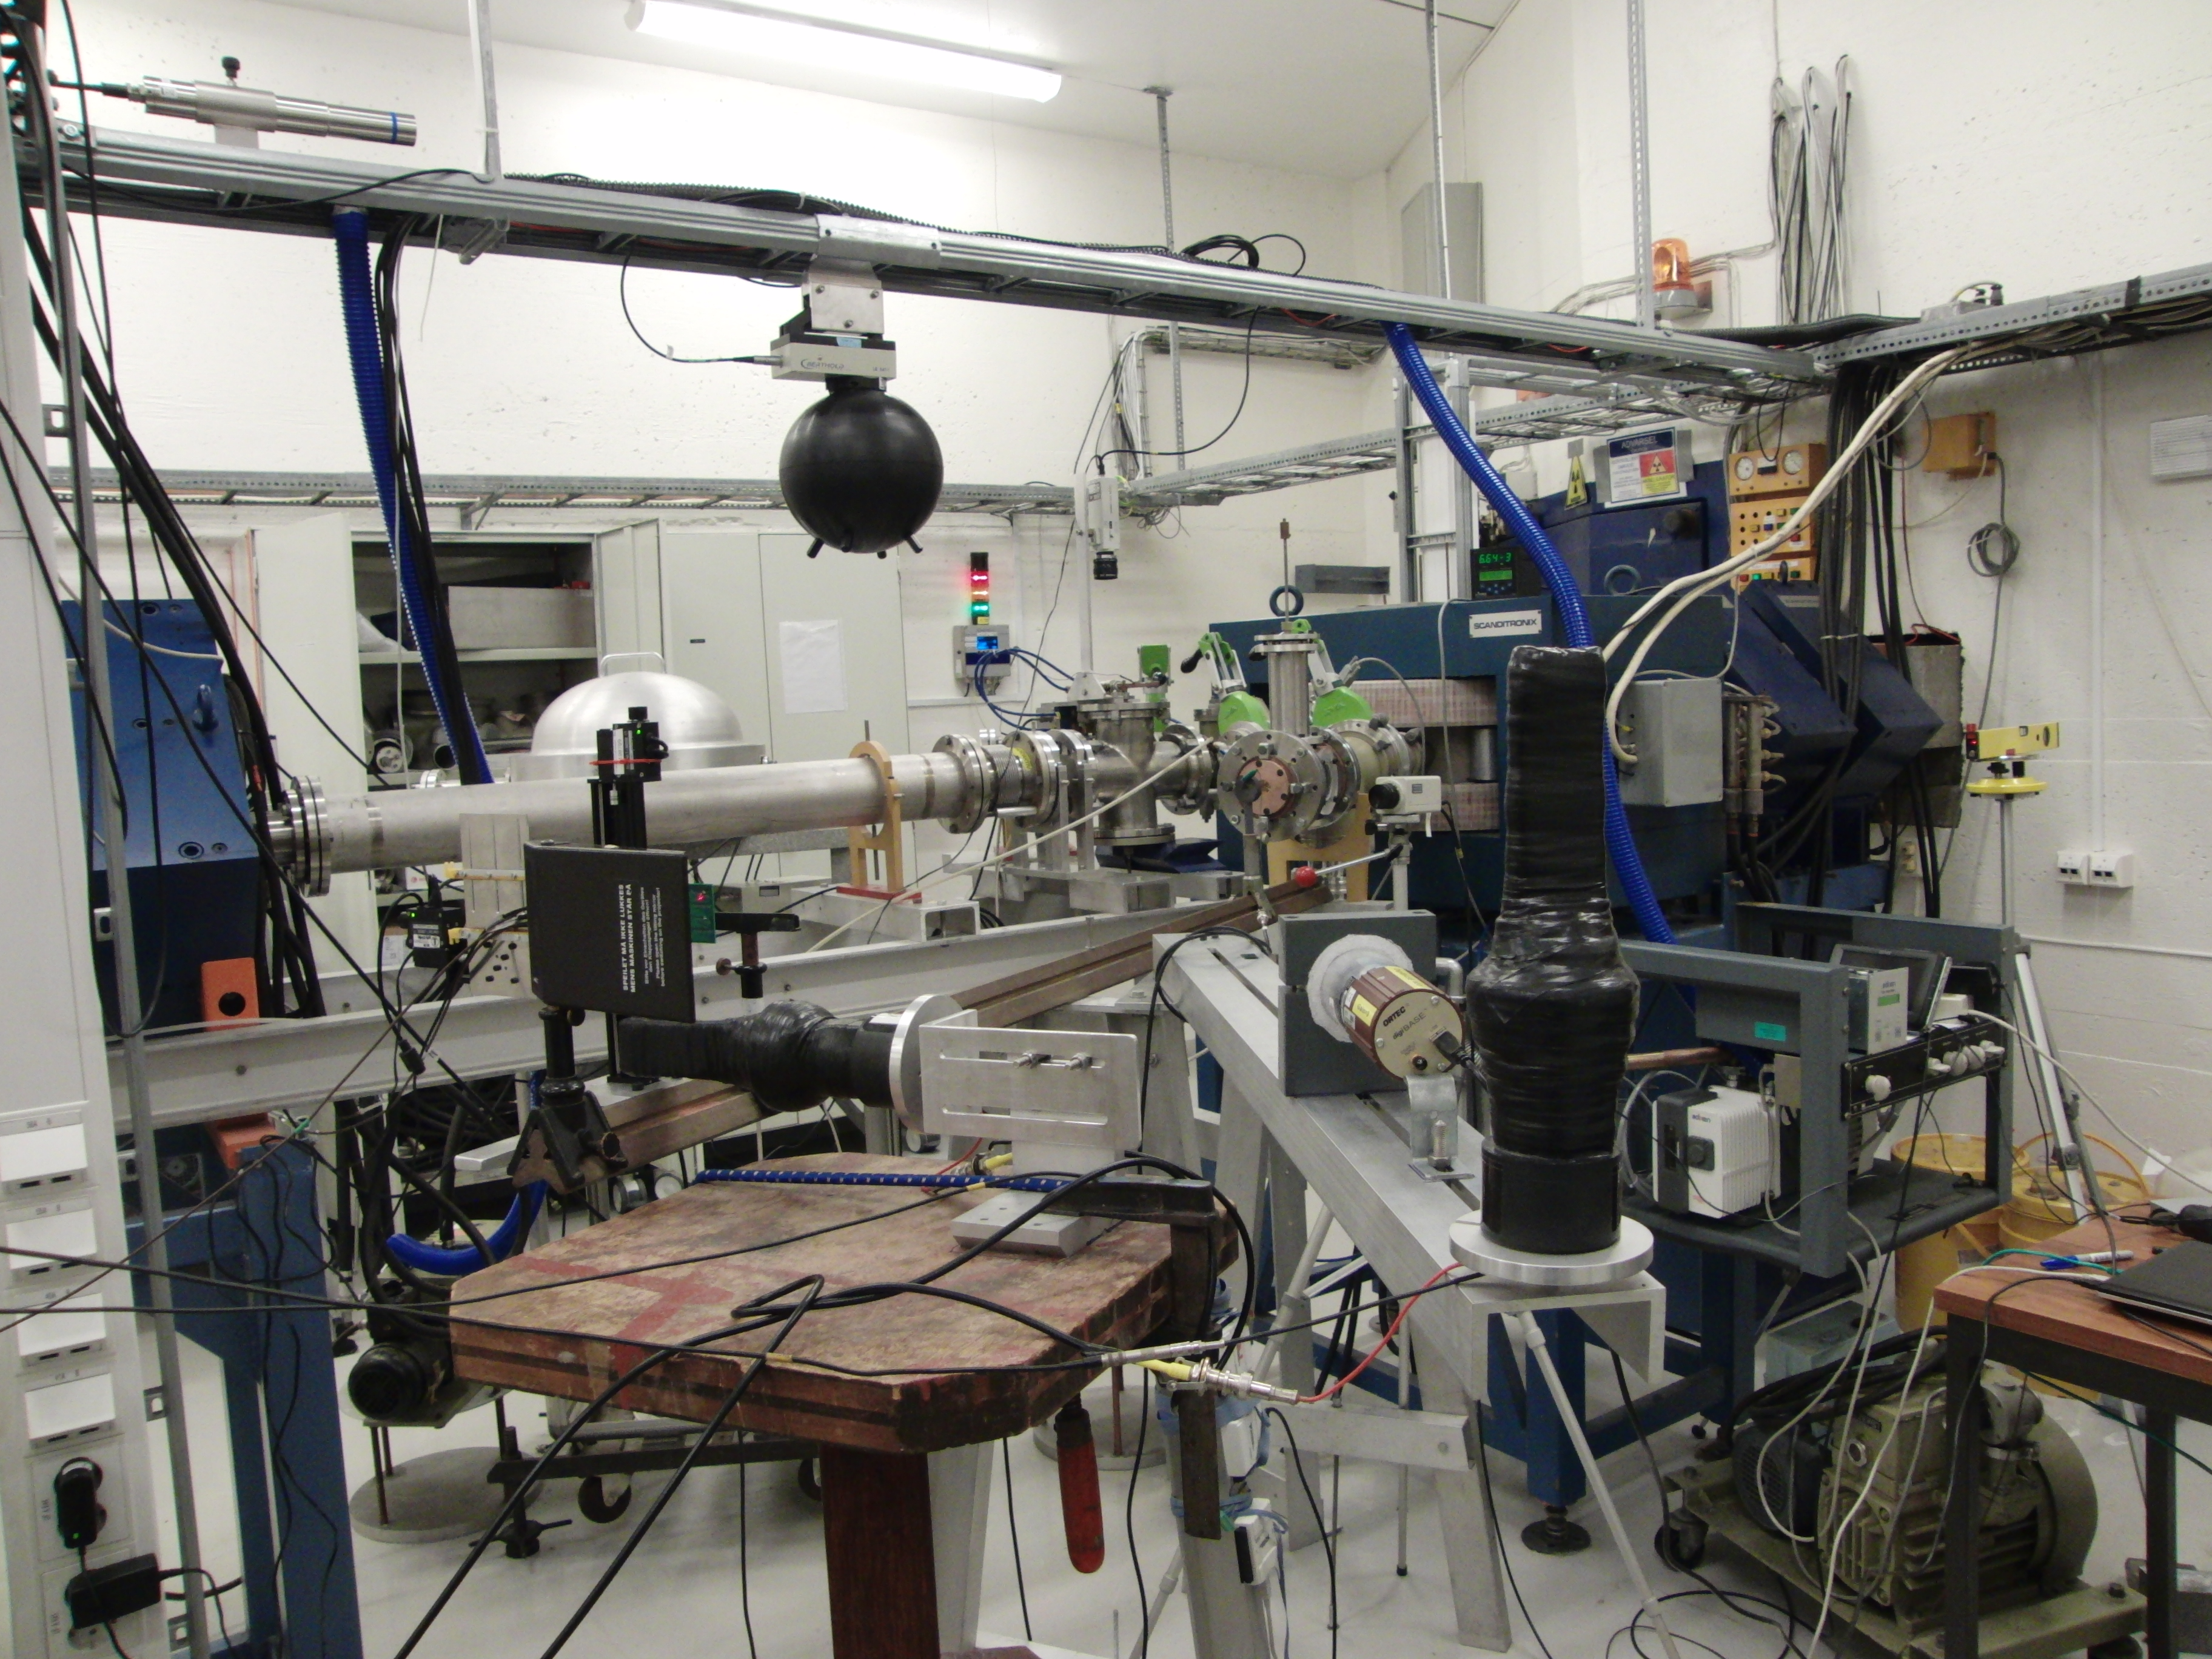
\includegraphics[width=\textwidth]{experiment_area.jpg}
  \caption{Picture of the experimental area}
  \label{experiment_area}
\end{figure}


\newpage
\begin{table}[h]
 \centering
\begin{tabular}{|l|p{12cm}|}\hline
Equipment & Explanation  \\ \hline \hline
Scintillator & A plastic scintillator with photomultiplier, that was used to measure relative radiation. We had two of these, one that was placed right under DUT and one that was placed 75cm away from DUT. We only used one during the experiment.   \\ \hline
High voltage regulator & Voltage for the photomultiplier. 800V was used  \\ \hline
8 test boards &  TPS51200, MIC69302WU, SN74AVCB16245, SN74AVC2T245, QS3VH257, SY89831U, ADN2814 and MAX3748 \\ \hline 
SRAM-board  & A PCB board with 4 SRAM cells, that was used to characterise the beam and to measure scintillator counts \\ \hline
Computer  & A VPN connection was set on a computer inside the experimental hall, so we where able to control the experiment outside the experimental hall. The computer was running LabView to control the experiment, data was also saved on the computer\\ \hline
USB DAQ  & Used to get analog and digital connection to the test boards and send data to the computer. \\ \hline
Radiation film  & A film that reacts when radiated with protons. Used to identify the beam. \\ \hline
Counting controller  & a device that counts rising or falling edges \\ \hline
leveled laser  & This was used to pinpoint the center of the beam.\\ \hline
Mirror & Reflecting the laser beam to the backside of the test boards.\\ \hline
XY-controller  & Connected to the computer so we can do minor changes to the placement of the test boards outside the experimental area\\ \hline
\end{tabular}
\caption{Equipment used in the experiment}
\label{equipment}
\end{table}

\subsection{Measurement equipment and test boards}
\subsubsection{SRAM}
The SRAM board consist of several SRAM chips and a flash based FPGA and some connections and supporting electronics. 
%A known pattern is written to the SRAM chips, and this pattern are constantly checked with the FPGA. 
When a SRAM chip is exposed to radiation a Single Event Upset(SEU) can occur.
The method of detecting an Single Event Upset (SEU) in a SRAM is rather straight
forward, as can be seen in the flow diagram of figure \ref{flowchart}. There is an initial startup
phase where a known pattern is written to all the addresses in the SRAM. When
the startup phase is done, the value from the first address is read back and compared
to a known value by xoring the known value with the read. If they are not alike a SEU has occurred,
and a 1 will return from the xor and be added to a SEU counter.
The correct value is then written back to the address and the system moves on to the next address.
  
A checkerboard pattern, a pattern of alternating ones and zeros, is used when writing
to the SRAM. To check for stuck bits, the bit pattern in the whole address space is inverted after each read. 
The cross section for SEU and particles is known through earlier experiment with the SRAM-board,
and is found to be $\unit{1.14\e{-6}}{\centi\square\meter}$.
The FPGA on the SRAM PCB is designed with RS485 two-way communication which makes it possible to edit firmware as well as sending data out. 
Through the experiment the SRAM PCB was connected with RS485 to a `en box som arild hadde` that could be connected to a computer. On the computer we run a LabVIEW program, that made us able to monitor data, as well as doing some settings. 
The SRAM board also had an input for scintillator counts, so we could monitor scintillator counts by the use of this board.

\begin{figure}[h]
  \centering
  \includegraphics[height=8cm, width=4cm]{SRAM_flowchart.png}
  \caption{Flowchart for SEU detection}
  \label{flowchart}
\end{figure}

\subsubsection{Scintillator}
The detection of ionizing radiation by the scintillation light produced in certain materials is one of the oldest techniques on record. In Geiger and Marsden�s famous scattering experiment of a-particles off Gold nuclei, the scattered a�s were observed via the scintillation light they produced when they hit a ZnS-screen. ZnS produced light flashes, called scintillation light, when hit by an $\alpha$. The scintillation process remains one of the most useful methods available for the detection and spectroscopy of a wide assortment of radiation.

\begin{figure}[h]
  \centering
  \includegraphics[width=\textwidth]{scintillator.png}
  \caption{Concept drawing of scintillator}
  \label{scintillator}
\end{figure}

\newpage

\subsubsection{The test boards}
TPS51200 -
A Sink/Source DDR termination regulator. Used to power DDR RAMs. We are going to use this for 0.75V DDR3 RAM.
\newline
MIC69302WU -
This is a high current low voltage regulator. Is going to be used to produce a 1.2V voltage.
\newline
SN74AVCB16245 -
This is a 16-bit noninverting bus transceiver, with configurable voltage transceiver and 3-state outputs.
\newline
SN74AVC2T245 -
This is a dual-bit noninverting bus transceiver ,with configurable voltage transceiver and 3-state outputs
\newline
QS3VH257 -
This is a Quad 2:1 multiplexer/demultiplexer with high bandwidth bus switch
\newline
SY89831U -
This is a high speed, 2$\giga\hertz$ differential LVPECL 1:4 fanout buffer optimized for ulta-low skew applications
\newline
ADN2814 -
This i a clock and data recovery IC with integrated Limiting amplifier. works in rate of 10Mb/s to 675 Mb/s.
\newline
MAX3748 -
This is a limiting amplifier. works in rate of 155Mb/s to 4.25Gb/s.

\newpage

\subsection{Preparation and characterization of the beam}
Before we could start testing the test boards, the cyclotron had to be made ready for a proton beam and the magnet controlling the direction had to be put in the right position to get the beam out in experiment area 2. This was done by the experienced lab personnel. 

\subsubsection{purpose of tests}
The purpose of testing these board is to see if they are able to survive in a highly radiated area.
Every IC that has been tested, are IC's that are going to be used in creation of the new RCU2 board, that is going to be placed in ALICE at CERN.


\subsubsection{Beam setup}
When the beam was set, we could start the characterization of the beam.
The first thing to do is to get an understanding of the beam,
too see that it is centered and that it hits around the area that we expect.
This was done by using radiation films that turns black when exposed to radiation. 
We put one of these right in front of the beam exit and one in front of DUT-area to see how the beam looks like at the two places.
This gave us a hunch of where the beam goes. A more precise calibration was done by the use of the SRAM board and the scintillator. 
By measuring the relation between scintillator counts on the scintillator which was in a locked position and SEU on the SRAM that was connected to a XY-controller(which made the SRAM freely to move), we were able to find a more precise position of the beam center by seeing which position gives most SEU compared to scintillator counts.

This had to be done everyday at startup before we could start the tests.
When the beam center is found and everything looks fine, the laser was placed in a position so the laser points to where we have found the center of the beam to be. After that we could switch out the SRAM board with the PCB that we were going to test. We were able to control the intensity of the beam freely from the control room inside the limitation of the beam (for protons that is up to 100$\micro\ampere$). This way we could control the dose of radiation we were giving to the test boards. The beam intensity could be measured with a Faraday Cup(FC), by putting it in front of the beam. But the FC had to be removed when we were doing tests, since it will block the beam.

\subsubsection{The test procedure}
Before the test day I had made simple test program in LabVIEW for each PCB that we were going to test.
Each PCB had a mark on the back indicating the center of the IC.
The PCB picked out for testing was placed in so that the laser pinpoint this mark, then the IC should be in the center of the beam.
We were running 3 labVIEW programs through the experiment, one for controlling the XY-controller,
one for SRAM PCB(for scintillator counts) and one program for each of the test boards.
The SRAM and test board programs were constantly saving data on the disk.

\section{Results and calculations from beam test at OCL}
The radiation was done in 5 days divided in two periodes 13.11-15.11 and 28.11-29.11. There had been made two version of most of the boards, the exception is TPS51200, ADN2814 and MAX3748 which I only made one version of.

A complete result of the tests can be found in one of the appendix.



\end{document}